% =====================================================================
% preview_gate_status_incomplete -- R/ggplot2 -> tikzDevice (Frame-A, ESWA target)
% Canonical-JSON-only. Regenerate: Rscript submissions/frame-a-eswa/figures-r/make_figures_frame_a.R
% Provenance (JSON path :: field = plotted value), one line per series:
% SOURCE: results/frame_a/cells/ :: real MIX_A cell count = 33.0000
% SOURCE: results/frame_a/cells/ :: real MIX_B cell count = 18.0000
% SOURCE: results/frame_a/cells/ :: real MIX_C cell count = 0.0000
% =====================================================================
% WARNING: QA-PREVIEW-NOT-FOR-SUBMISSION (generated 2026-07-23 08:37:32 EDT)
% This file is NOT camera-ready. The MIX_A preview under figures-qa/
% !TEX encoding = UTF-8 Unicode
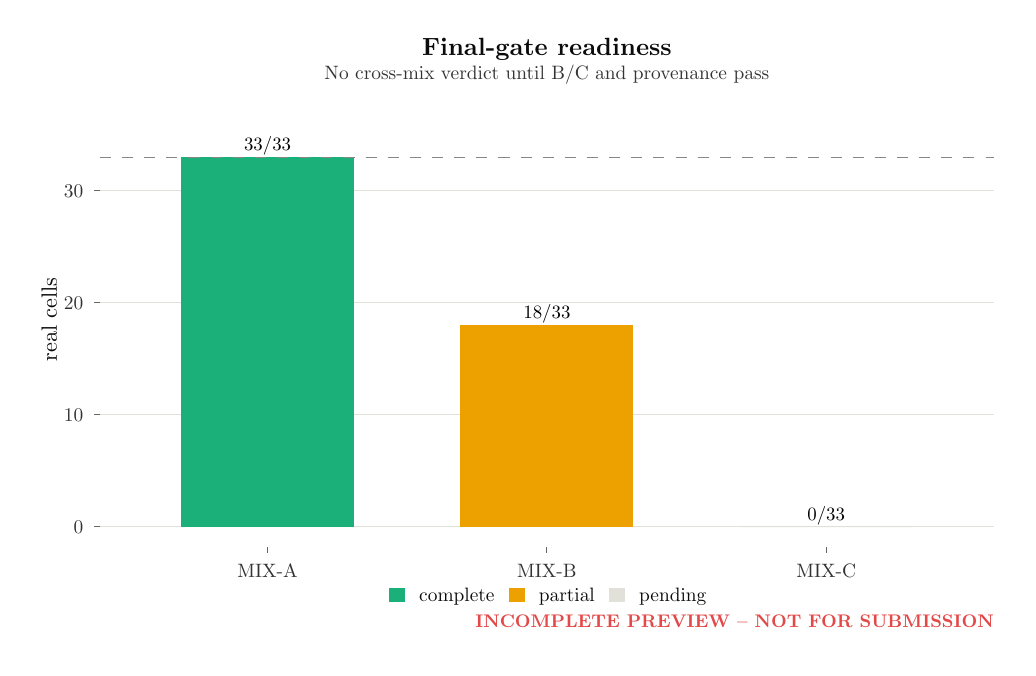
\begin{tikzpicture}[x=1pt,y=1pt]
\definecolor{fillColor}{RGB}{255,255,255}
\path[use as bounding box,fill=fillColor,fill opacity=0.00] (0,0) rectangle (354.12,224.04);
\begin{scope}
\path[clip] (  0.00,  0.00) rectangle (354.12,224.04);
\definecolor{fillColor}{RGB}{255,255,255}

\path[fill=fillColor] ( -0.00,  0.00) rectangle (354.12,224.04);
\end{scope}
\begin{scope}
\path[clip] ( 26.11, 36.25) rectangle (349.12,200.89);
\definecolor{drawColor}{RGB}{225,224,217}

\path[draw=drawColor,line width= 0.3pt,line join=round] ( 26.11, 43.74) --
	(349.12, 43.74);

\path[draw=drawColor,line width= 0.3pt,line join=round] ( 26.11, 84.19) --
	(349.12, 84.19);

\path[draw=drawColor,line width= 0.3pt,line join=round] ( 26.11,124.64) --
	(349.12,124.64);

\path[draw=drawColor,line width= 0.3pt,line join=round] ( 26.11,165.09) --
	(349.12,165.09);
\definecolor{fillColor}{RGB}{27,175,122}

\path[fill=fillColor] ( 55.39, 43.74) rectangle (117.97,177.23);
\definecolor{fillColor}{RGB}{237,161,0}

\path[fill=fillColor] (156.33, 43.74) rectangle (218.91,116.55);
\definecolor{fillColor}{RGB}{225,224,217}

\path[fill=fillColor] (257.27, 43.74) rectangle (319.85, 43.74);
\definecolor{drawColor}{RGB}{137,135,129}

\path[draw=drawColor,line width= 0.5pt,dash pattern=on 4pt off 4pt ,line join=round] ( 26.11,177.23) -- (349.12,177.23);
\definecolor{drawColor}{RGB}{0,0,0}

\node[text=drawColor,anchor=base,inner sep=0pt, outer sep=0pt, scale=  0.68] at ( 86.68,179.58) {33/33};

\node[text=drawColor,anchor=base,inner sep=0pt, outer sep=0pt, scale=  0.68] at (187.62,118.90) {18/33};

\node[text=drawColor,anchor=base,inner sep=0pt, outer sep=0pt, scale=  0.68] at (288.56, 46.09) {0/33};
\end{scope}
\begin{scope}
\path[clip] (  0.00,  0.00) rectangle (354.12,224.04);
\definecolor{drawColor}{gray}{0.20}

\node[text=drawColor,anchor=base east,inner sep=0pt, outer sep=0pt, scale=  0.70] at ( 20.06, 41.32) {0};

\node[text=drawColor,anchor=base east,inner sep=0pt, outer sep=0pt, scale=  0.70] at ( 20.06, 81.78) {10};

\node[text=drawColor,anchor=base east,inner sep=0pt, outer sep=0pt, scale=  0.70] at ( 20.06,122.23) {20};

\node[text=drawColor,anchor=base east,inner sep=0pt, outer sep=0pt, scale=  0.70] at ( 20.06,162.68) {30};
\end{scope}
\begin{scope}
\path[clip] (  0.00,  0.00) rectangle (354.12,224.04);
\definecolor{drawColor}{gray}{0.40}

\path[draw=drawColor,line width= 0.3pt,line join=round] ( 24.11, 43.74) --
	( 26.11, 43.74);

\path[draw=drawColor,line width= 0.3pt,line join=round] ( 24.11, 84.19) --
	( 26.11, 84.19);

\path[draw=drawColor,line width= 0.3pt,line join=round] ( 24.11,124.64) --
	( 26.11,124.64);

\path[draw=drawColor,line width= 0.3pt,line join=round] ( 24.11,165.09) --
	( 26.11,165.09);
\end{scope}
\begin{scope}
\path[clip] (  0.00,  0.00) rectangle (354.12,224.04);
\definecolor{drawColor}{gray}{0.40}

\path[draw=drawColor,line width= 0.3pt,line join=round] ( 86.68, 34.25) --
	( 86.68, 36.25);

\path[draw=drawColor,line width= 0.3pt,line join=round] (187.62, 34.25) --
	(187.62, 36.25);

\path[draw=drawColor,line width= 0.3pt,line join=round] (288.56, 34.25) --
	(288.56, 36.25);
\end{scope}
\begin{scope}
\path[clip] (  0.00,  0.00) rectangle (354.12,224.04);
\definecolor{drawColor}{gray}{0.20}

\node[text=drawColor,anchor=base,inner sep=0pt, outer sep=0pt, scale=  0.70] at ( 86.68, 25.38) {MIX-A};

\node[text=drawColor,anchor=base,inner sep=0pt, outer sep=0pt, scale=  0.70] at (187.62, 25.38) {MIX-B};

\node[text=drawColor,anchor=base,inner sep=0pt, outer sep=0pt, scale=  0.70] at (288.56, 25.38) {MIX-C};
\end{scope}
\begin{scope}
\path[clip] (  0.00,  0.00) rectangle (354.12,224.04);
\definecolor{drawColor}{RGB}{11,11,11}

\node[text=drawColor,rotate= 90.00,anchor=base,inner sep=0pt, outer sep=0pt, scale=  0.80] at ( 10.51,118.57) {real cells};
\end{scope}
\begin{scope}
\path[clip] (  0.00,  0.00) rectangle (354.12,224.04);
\definecolor{fillColor}{RGB}{27,175,122}

\path[fill=fillColor] (130.57, 16.42) rectangle (136.41, 21.44);
\end{scope}
\begin{scope}
\path[clip] (  0.00,  0.00) rectangle (354.12,224.04);
\definecolor{fillColor}{RGB}{237,161,0}

\path[fill=fillColor] (173.79, 16.42) rectangle (179.63, 21.44);
\end{scope}
\begin{scope}
\path[clip] (  0.00,  0.00) rectangle (354.12,224.04);
\definecolor{fillColor}{RGB}{225,224,217}

\path[fill=fillColor] (210.03, 16.42) rectangle (215.86, 21.44);
\end{scope}
\begin{scope}
\path[clip] (  0.00,  0.00) rectangle (354.12,224.04);
\definecolor{drawColor}{RGB}{11,11,11}

\node[text=drawColor,anchor=base west,inner sep=0pt, outer sep=0pt, scale=  0.70] at (141.49, 16.52) {complete};
\end{scope}
\begin{scope}
\path[clip] (  0.00,  0.00) rectangle (354.12,224.04);
\definecolor{drawColor}{RGB}{11,11,11}

\node[text=drawColor,anchor=base west,inner sep=0pt, outer sep=0pt, scale=  0.70] at (184.71, 16.52) {partial};
\end{scope}
\begin{scope}
\path[clip] (  0.00,  0.00) rectangle (354.12,224.04);
\definecolor{drawColor}{RGB}{11,11,11}

\node[text=drawColor,anchor=base west,inner sep=0pt, outer sep=0pt, scale=  0.70] at (220.94, 16.52) {pending};
\end{scope}
\begin{scope}
\path[clip] (  0.00,  0.00) rectangle (354.12,224.04);
\definecolor{drawColor}{gray}{0.20}

\node[text=drawColor,anchor=base,inner sep=0pt, outer sep=0pt, scale=  0.70] at (187.62,205.26) {No cross-mix verdict until B/C and provenance pass};
\end{scope}
\begin{scope}
\path[clip] (  0.00,  0.00) rectangle (354.12,224.04);
\definecolor{drawColor}{RGB}{11,11,11}

\node[text=drawColor,anchor=base,inner sep=0pt, outer sep=0pt, scale=  0.90] at (187.62,213.83) {\bfseries Final-gate readiness};
\end{scope}
\begin{scope}
\path[clip] (  0.00,  0.00) rectangle (354.12,224.04);
\definecolor{drawColor}{RGB}{227,73,72}

\node[text=drawColor,anchor=base east,inner sep=0pt, outer sep=0pt, scale=  0.66] at (349.12,  7.28) {\bfseries INCOMPLETE PREVIEW -- NOT FOR SUBMISSION};
\end{scope}
\end{tikzpicture}
